\section{Rezultaty i wnioski}

<Podrozdziały: "Funkcjonowanie algorytmu G-średnich", "Funkcjonowanie algorytmu SVM">

Pomiary czasu wykonywania programów napisanych w poszczególnych językach dla różnych paczek danych z bazy MIT-BIH zostały przedstawione w Tab.\ref{tabResults}.

\begin{table}[!tp]
	\centering
	\caption{Czasy wykonywania programu w poszczególnych językach dla różnych paczek danych. Wyniki wyrażone w sekundach}
	\label{tabResults}
	\begin{tabular}{|c|c|c|c|c|}
		\hline
		Nr paczki z MIT-BIH & C++ & Matlab & Python & Julia\\ \hline		
		100 & 2.78424 & 1.9523 & 12.815439 & 5.901852174\\ \hline
		101 & 2.46179 & 1.4195 & 10.492137 & 1.899932399\\ \hline
		102 & 2.73843 & 1.2609 & 12.242185 & 2.215825099\\ \hline
		103 & 3.23737 & 2.3951 & 11.708208 & 2.179983401\\ \hline
		104 & 2.67691 & 1.6457 & 11.895952 & 2.133522994\\ \hline
		105 & 3.49907 & 1.3186 & 14.702323 & 3.123101161\\ \hline
		106 & 2.31706 & 1.8217 & 10.365989 & 2.114899549\\ \hline
		107 & 2.29397 & 1.5331 &  9.988119 & 2.069017174\\ \hline
		108 & 1.91518 & 1.7391 &  8.503747 & 2.10760114\\ \hline
		109 & 3.23669 & 1.2506 & 13.910034 & 3.42160439\\ \hline
		111 & 2.65892 & 1.8369 & 11.575133 & 2.874097787\\ \hline
		112 & 3.23952 & 2.2931 & 14.707609 & 3.345013555\\ \hline
		113 & 2.38218 & 1.2857 & 10.2796   & 1.938375007\\ \hline
		114 & 1.28468 & 0.5056 &  5.547578 & 1.534204408\\ \hline
		115 & 2.75770 & 1.2325 & 11.059755 & 2.207411682\\ \hline
		116 & 3.69870 & 1.242  & 13.344349 & 2.587637119\\ \hline
		117 & 2.15060 & 1.506  &  8.462129 & 1.643660476\\ \hline
		119 & 8.40456 & 1.5771 & 10.99204  & 2.071278448\\ \hline
		121 & 2.47024 & 2.0902 & 10.279925 & 1.976437859\\ \hline
		122 & 4.07225 & 2.0928 & 14.211312 & 3.117896543\\ \hline
		123 & 2.07675 & 0.7942 &  8.39699  & 1.721477354\\ \hline
		124 & 1.97200 & 1.6778 &  8.137572 & 1.714434604\\ \hline
		200 & 2.58850 & 1.8849 & 11.517102 & 2.827846386\\ \hline
		201 & 2.35619 & 1.8963 &  9.249272 & 1.864559098\\ \hline
		202 & 2.70065 & 2.132  & 13.789148 & 3.778367525\\ \hline
		203 & 3.10119 & 1.2565 & 14.579523 & 3.147122344\\ \hline
		205 & 3.30010 & 1.3475 & 15.066897 & 3.260278958\\ \hline
		208 & 4.41398 & 2.4411 & 15.573072 & 3.529202731\\ \hline
		209 & 3.99421 & 2.139  & 17.397029 & 4.002761863\\ \hline	
		210 & 3.23209 & 1.1721 & 26.913411 & 6.433184431\\ \hline
		212 & 3.59817 & 2.9475 & 26.890231 & 3.390088991\\ \hline
		213 & 4.19173 & 2.3988 & 31.479429 & 4.146098275\\ \hline
		214 & 2.65823 & 1.8288 & 18.571949 & 2.420839058\\ \hline
		215 & 4.51468 & 1.6584 & 30.439442 & 3.954894738\\ \hline
		217 & 2.53682 & 2.0103 & 18.701152 & 2.587683551\\ \hline
		219 & 2.82458 & 1.8043 & 19.748443 & 3.281731301\\ \hline
		220 & 2.70177 & 1.2670 & 18.710136 & 2.665970912\\ \hline		
		221 & 3.06091 & 1.7631 & 13.708571 & 3.006166138\\ \hline
		222 & 3.14592 & 1.2655 & 14.3837   & 3.223767787\\ \hline
		223 & 3.08768 & 1.2356 & 13.731657 & 3.006029445\\ \hline
		230 & 2.78232 & 1.8286 & 14.19151  & 2.875082168\\ \hline
		231 & 2.08884 & 1.4458 &  8.698872 & 3.391200109\\ \hline
		232 & 2.26944 & 1.3707 & 10.32135  & 2.354562975\\ \hline
		233 & 3.47059 & 2.5759 & 15.583746 & 3.477575961\\ \hline
		234 & 3.39626 & 3.6223 & 16.492193 & 3.583639883\\ \hline
	\end{tabular}
\end{table}

\begin{table}[!tp]
	\centering
	\caption{Liczby klas wyliczonych przez G-means}
	\label{tabResults2}
	\begin{tabular}{|c|c|c|c|}
		\hline
		Nr paczki z MIT-BIH & Matlab & Python & Julia\\ \hline		
		100 & 16 & 16 & 16\\ \hline
		101 & 14 & 16 & 16\\ \hline
		102 & 14 & 16 & 16\\ \hline
		103 & 27 & 16 & 16\\ \hline
		104 & 29 & 16 & 16\\ \hline
		105 &  1 & 20 & 20\\ \hline
		106 & 35 & 16 & 16\\ \hline
		107 & 31 & 16 & 16\\ \hline
		108 & 32 & 15 & 15\\ \hline
		109 &  1 & 21 & 21\\ \hline
		111 & 22 & 17 & 17\\ \hline
		112 & 15 & 19 & 19\\ \hline
		113 & 13 & 16 & 16\\ \hline
		114 &  1 & 15 & 15\\ \hline
		115 & 15 & 16 & 16\\ \hline
		116 &  1 & 16 & 16\\ \hline
		117 & 23 & 16 & 16\\ \hline
		119 & 33 & 16 & 16\\ \hline
		121 & 27 & 16 & 16\\ \hline
		122 & 29 & 21 & 21\\ \hline
		123 &  1 & 16 & 16\\ \hline
		124 & 30 & 15 & 15\\ \hline
		200 & 32 & 20 & 20\\ \hline
		201 & 56 & 13 & 13\\ \hline
		202 & 29 & 21 & 21\\ \hline
		203 &  1 & 26 & 26\\ \hline
		205 &  1 & 21 & 21\\ \hline
		208 & 36 & 24 & 24\\ \hline
		209 & 21 & 31 & 31\\ \hline
		210 &  1 & 20 & 20\\ \hline
		212 & 18 & 25 & 25\\ \hline
		213 & 28 & 32 & 32\\ \hline
		214 & 33 & 18 & 18\\ \hline
		215 & 18 & 32 & 32\\ \hline
		217 & 65 & 17 & 17\\ \hline
		219 & 36 & 15 & 15\\ \hline
		220 & 22 & 16 & 16\\ \hline	
		221 & 33 & 19 & 19\\ \hline
		222 &  1 & 22 & 22\\ \hline
		223 &  1 & 18 & 18\\ \hline
		230 & 15 & 20 & 20\\ \hline
		231 & 39 & 12 & 12\\ \hline
		232 & 28 & 17 & 17\\ \hline
		233 & 42 & 24 & 24\\ \hline
		234 & 27 & 29 & 29\\ \hline
	\end{tabular}
\end{table}

Krótki czas wykonywania programu napisanego w Matlabie wynika głównie z wykorzystania biblioteki libsvm \cite{csie}, która jest napisana w C. Dla pozostałych języków zaimplementowano maszynę wektorów nośnych w oparciu o pliki źródłowe wspomnianej biblioteki.

Wykorzystanie metody SVM z szesnastoelementowym wektorem cech wydaje się złym rozwiązaniem, gdyż niemal zawsze wektor klasyfikowany jest do jednej klasy - patrz Rys.\ref{fig:hist1}. Poza zbyt licznym wektorem cech wpływ na to ma również fakt, że około 90\% zespołów QRS z bazy MIT-BIH reprezentują pobudzenia nadkomorowe. Rozwiązaniem problemu klasyfikacji może okazać się odpowiednie zmniejszenie liczności wykorzystywanego wektora cech.

Przeprowadzono również testy, w których SVM korzystał z różnych modeli (wygenerowanych z różnych paczek danych). Zaobserwowano, że normalizacja wektorów uczących znacznie przyspiesza proces uczenia, czego potwierdzeniem jest Rys.\ref{fig:SVM}.

\begin{figure}[!htp]
	\centering
	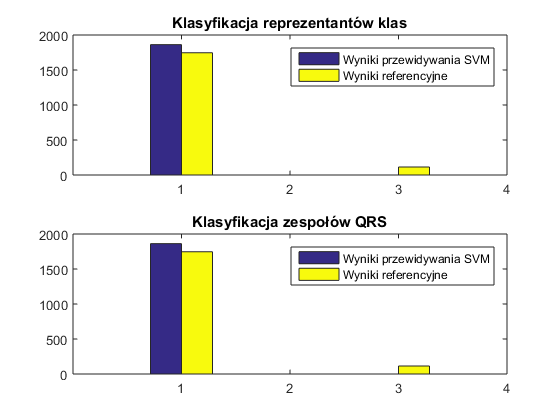
\includegraphics[width=15cm]{Grafika/101_2_3}
	\caption{Histogramy klasyfikacji zespołów dla paczki danych o numerze 101}
	\label{fig:hist1}
\end{figure}

\begin{figure}[!htp]
	\centering
	\includegraphics[width=15cm]{Grafika/SVMTrain}
	\caption{Wpływ normalizacji na czas nauki SVM}
	\label{fig:TrainNormSVM}
\end{figure}

<Coś o gmeans - że w C++ nie było, a tutaj jest>


%\begin{table}[H]
%\caption{Example table}
%\centering
%\begin{tabular}{llr}
%\toprule
%\multicolumn{2}{c}{Name} \\
%\cmidrule(r){1-2}
%First name & Last Name & Grade \\
%\midrule
%John & Doe & $7.5$ \\
%Richard & Miles & $2$ \\
%\bottomrule
%\end{tabular}
%\end{table}
